\section{\centering 附件}

\subsection{過去的募資經驗}
\label{fig:Appendix-fundraising}
\begin{figure}[H]
	\centering
	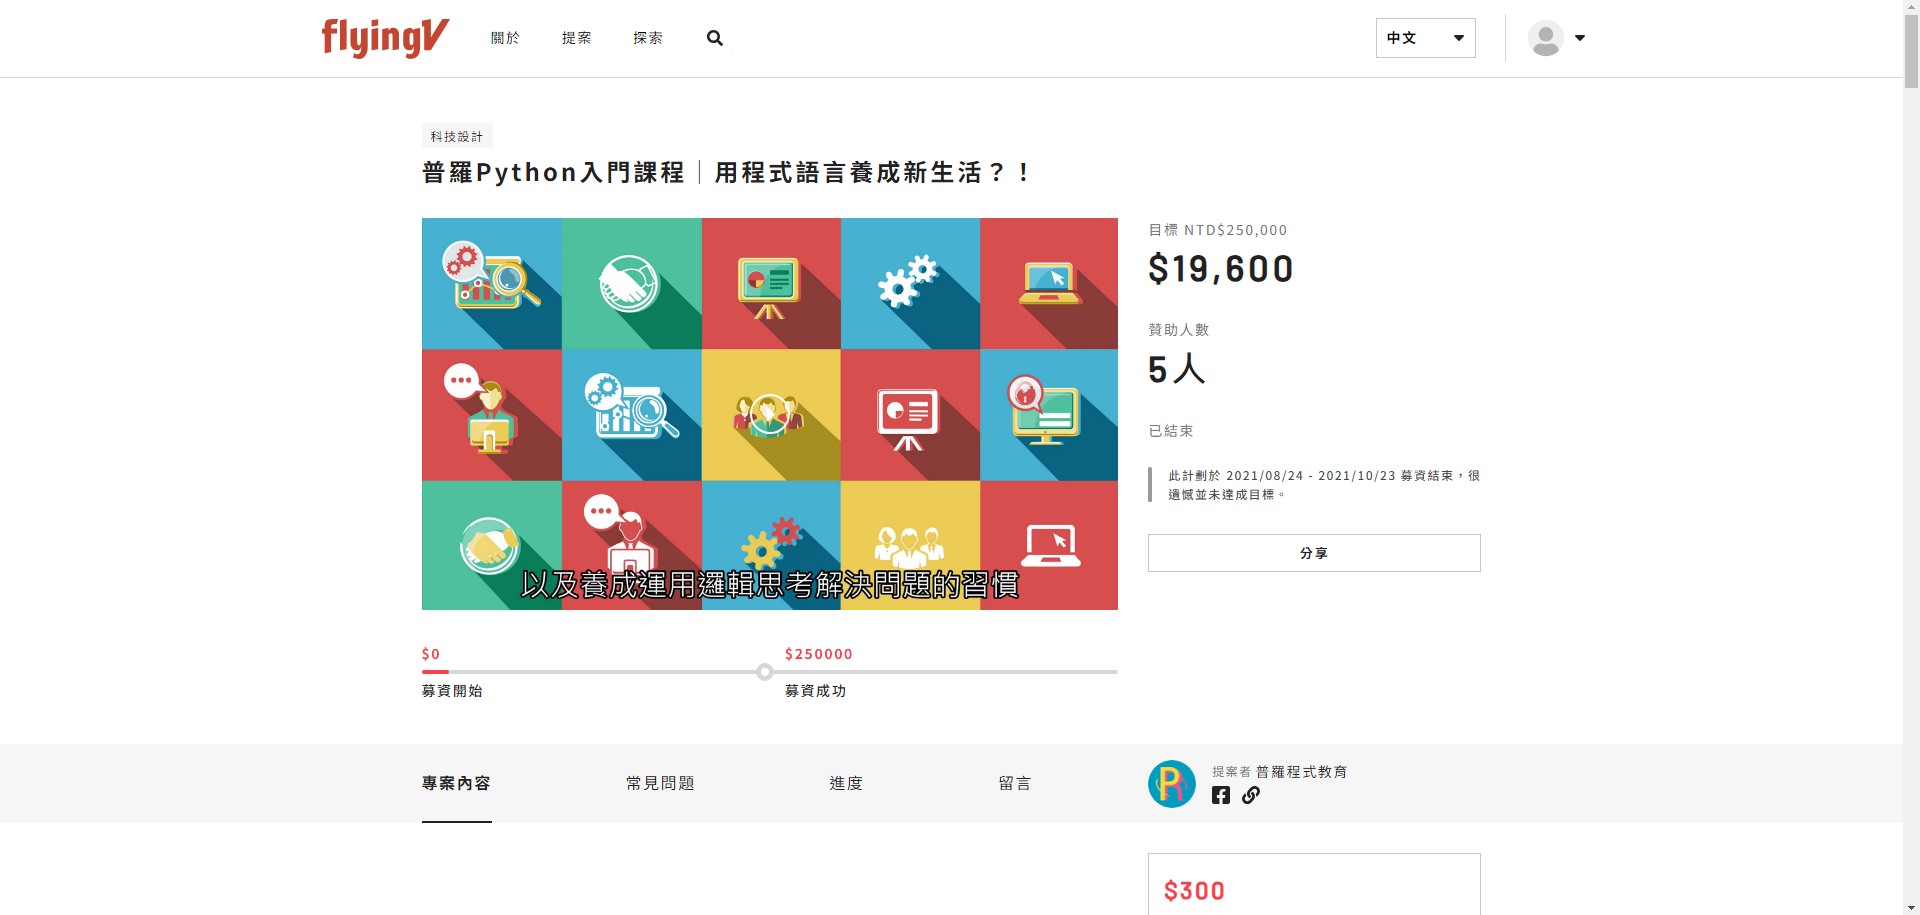
\includegraphics[width=0.8\textwidth]{images/flyingv-19600.png}
	\caption{flyingV群眾募資 - 成果}
	\label{fig:flyingv}
\end{figure}

\subsection{過去的創業研習經驗}
\label{fig:Appendix-Training}
\begin{figure}[H]
  \centering
  \begin{subfigure}{0.32\linewidth}
    \centering
    
\includegraphics[width=0.8\textwidth]{images/training-1.png}
    \caption{112 學年第一學期學生創業戰鬥營 - 林一}
    \label{fig:Training-1}
  \end{subfigure}
  \begin{subfigure}{0.32\linewidth}
    \centering
    
\includegraphics[width=0.8\textwidth]{images/training-2.png}
    \caption{112 學年第一學期學生創業新手村 - 簡蔚驊}
    \label{fig:Training-2}
  \end{subfigure}
  \begin{subfigure}{0.32\linewidth}
    \centering
    
\includegraphics[width=0.8\textwidth]{images/training-3.png}
    \caption{112 學年第一學期學生創業戰鬥 - 王裕傑}
    \label{fig:Training-3}
  \end{subfigure}
  \caption{過去的創業研習經驗}
\end{figure}

\subsection{過去的創業競賽經驗}
\label{fig:Appendix-Competition}
\begin{figure}[H]
	\centering
	\begin{subfigure}{0.45\linewidth}
		\centering
		
\includegraphics[width=0.6\textwidth]{images/competition-1.jpeg}
		\caption{2021武漢金銀湖盃第七屆海峽兩岸青年創新創業大賽入選台灣賽區菁英賽決賽}
		\label{fig:Competition-1}
	\end{subfigure}
	\begin{subfigure}{0.45\linewidth}
		\centering
		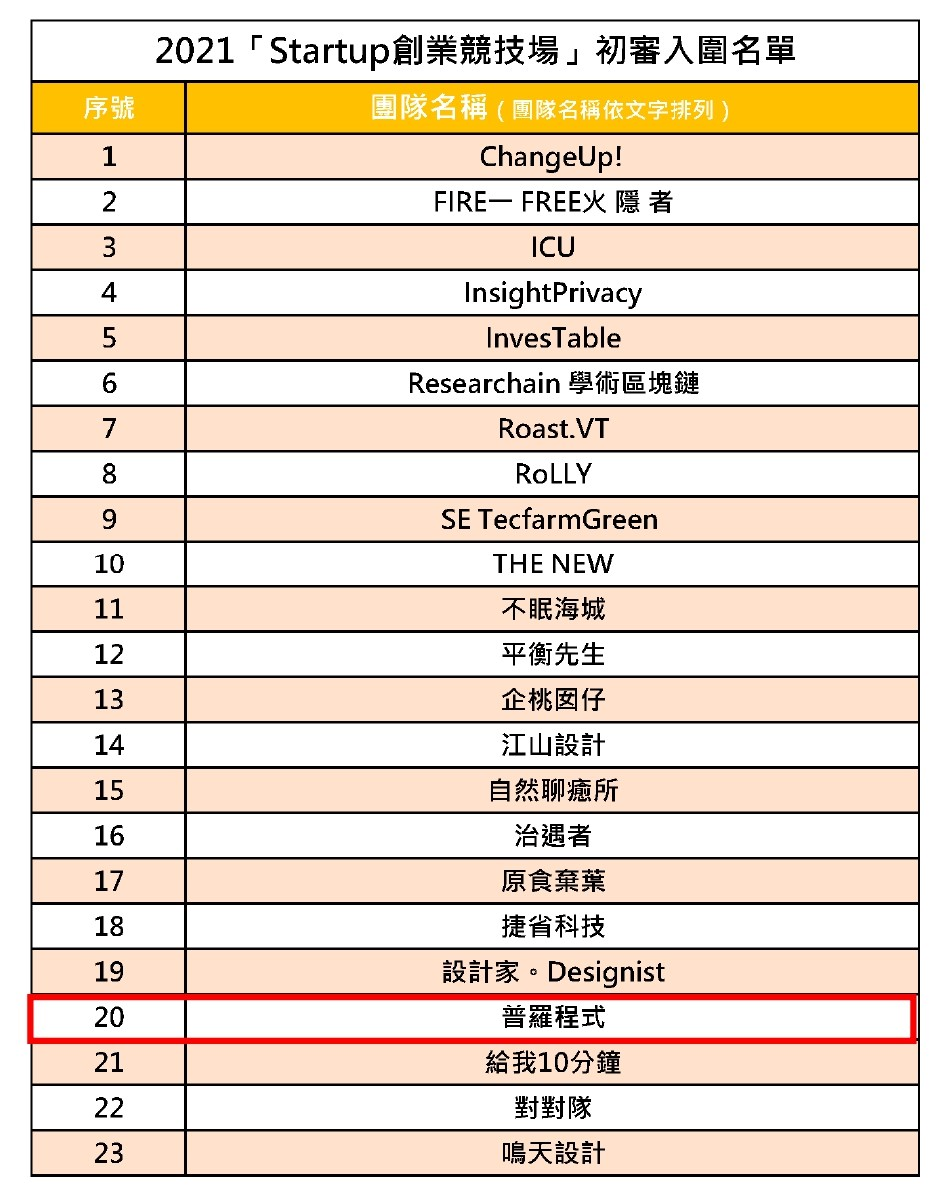
\includegraphics[width=0.6\textwidth]{images/competition-2.jpeg}
		\caption{2021師大Startup競技場決賽}
		\label{fig:Competition-2}
	\end{subfigure}
	\caption{過去的創業競賽經驗}
\end{figure}

\subsection{過去的行銷成果}
\label{fig:Appendix-Marketing}
\begin{figure}[H]
	\centering
	\begin{subfigure}{0.32\linewidth}
		\centering
		
\includegraphics[width=1\textwidth]{images/FB.png}
		\caption{Facebook}
		\label{fig:FB}
	\end{subfigure}
	\begin{subfigure}{0.32\linewidth}
		\centering
		
\includegraphics[width=0.6\textwidth]{images/IG.jpg}
		\caption{Instagram}
		\label{fig:IG}
	\end{subfigure}
	\begin{subfigure}{0.32\linewidth}
		\centering
		
\includegraphics[width=1\textwidth]{images/website.png}
		\caption{普羅官網}
		\label{fig:website}
	\end{subfigure}
	\caption[社群平台]{社群平台\\(資料來源:於2024年1月15日,截取自普羅Facebook、Instagram及官網)}
	\label{fig:platform}
\end{figure}

\subsection{各平台教師數量}
\label{fig:Appendix-Teacher}
% 三張圖
\begin{figure}[H]
	\centering
	\begin{subfigure}{0.32\linewidth}
		\centering
		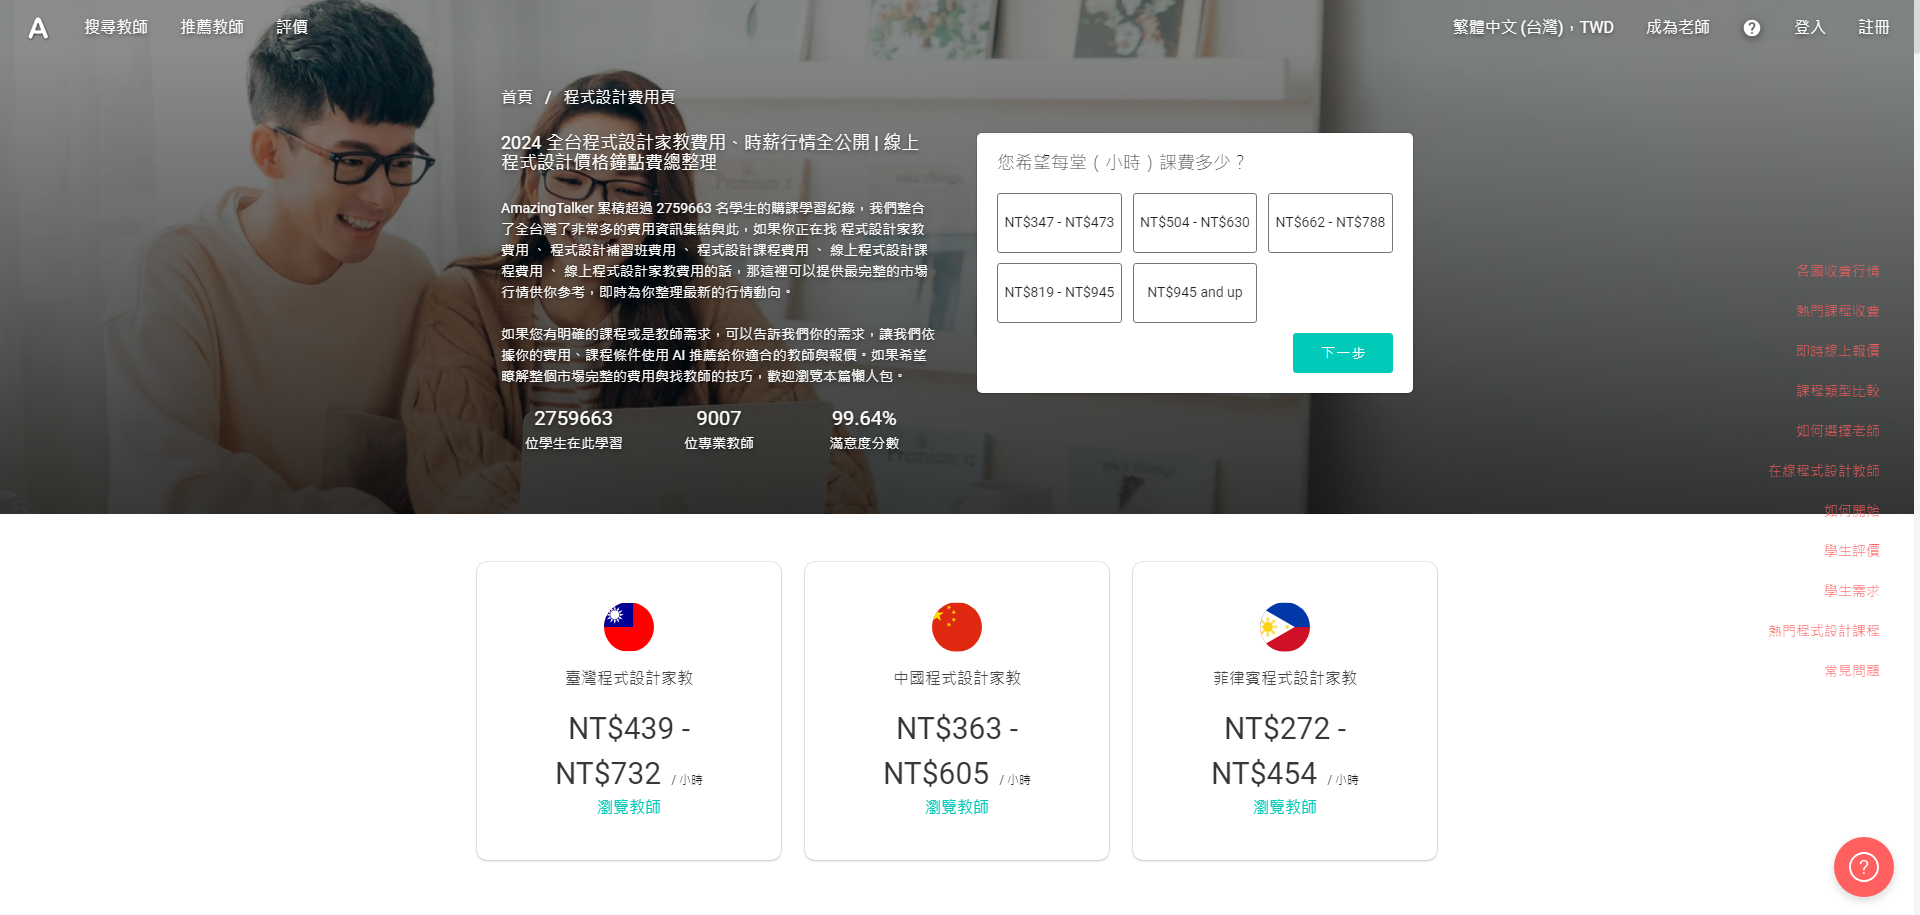
\includegraphics[width=1\textwidth]{images/A-9007.png}
		\caption{AmazingTalker線上家教平台}
		\label{fig:Teacher-1}
	\end{subfigure}
	\begin{subfigure}{0.32\linewidth}
		\centering
		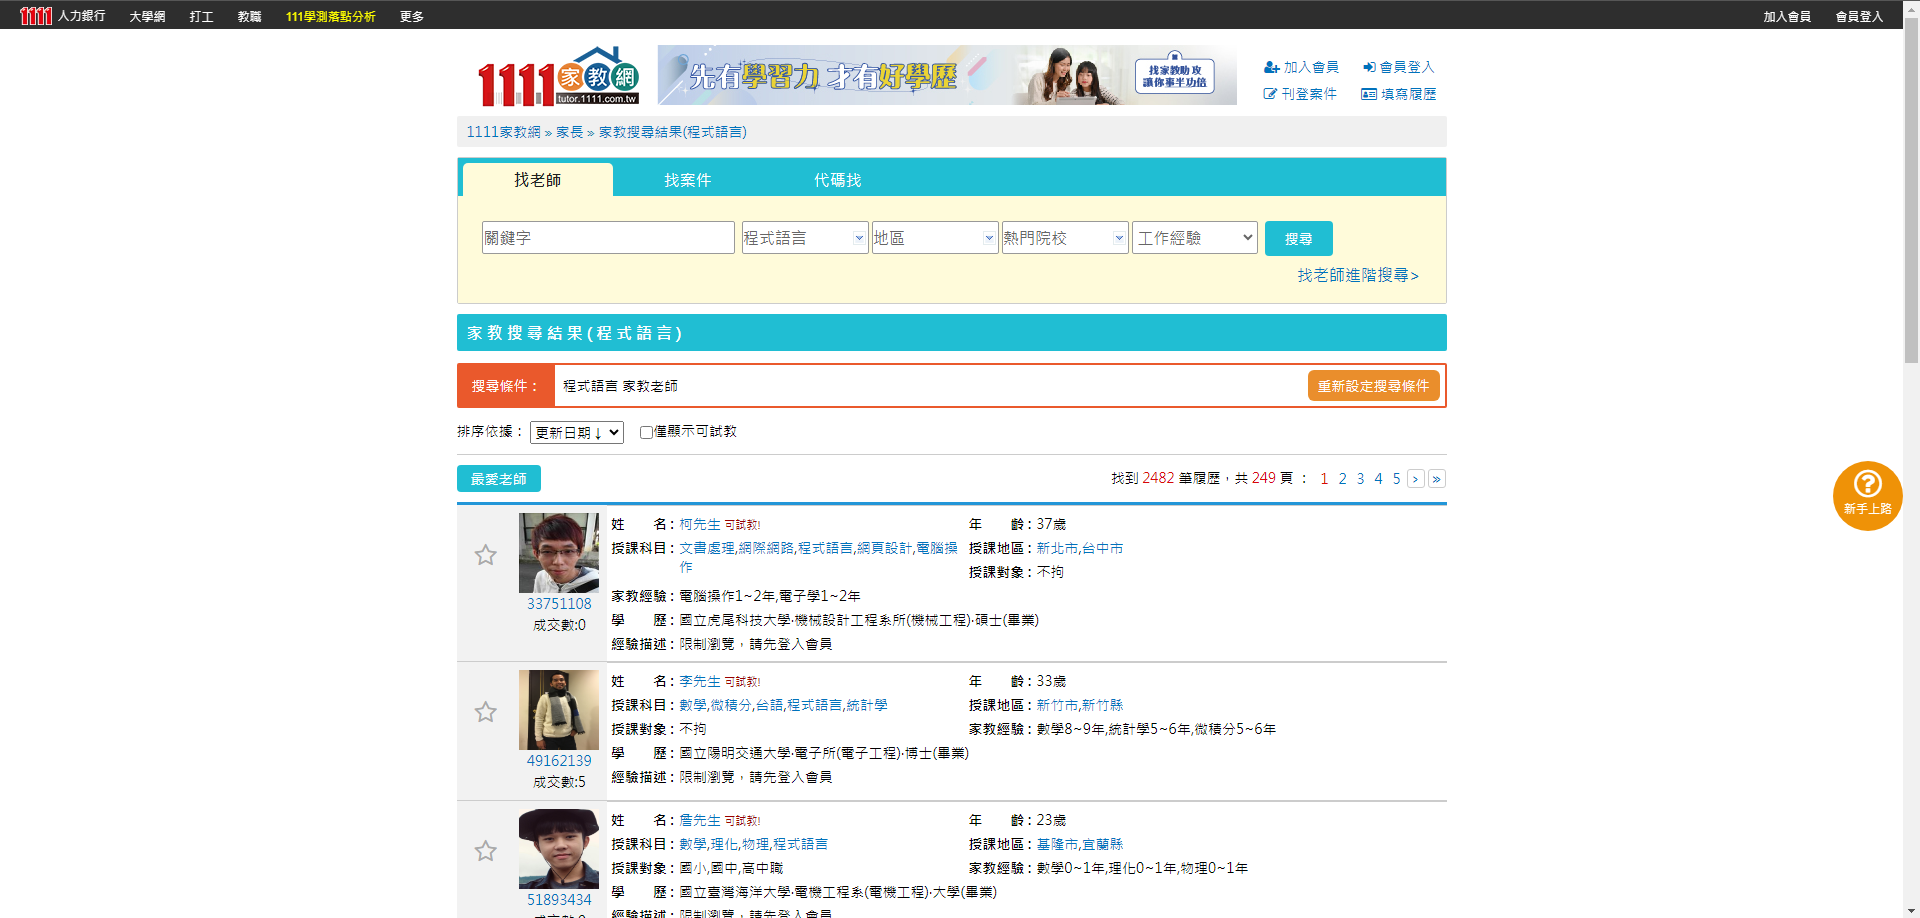
\includegraphics[width=1\textwidth]{images/1111-2482.png}
		\caption{1111家教網}
		\label{fig:Teacher-2}
	\end{subfigure}
	\begin{subfigure}{0.32\linewidth}
		\centering
		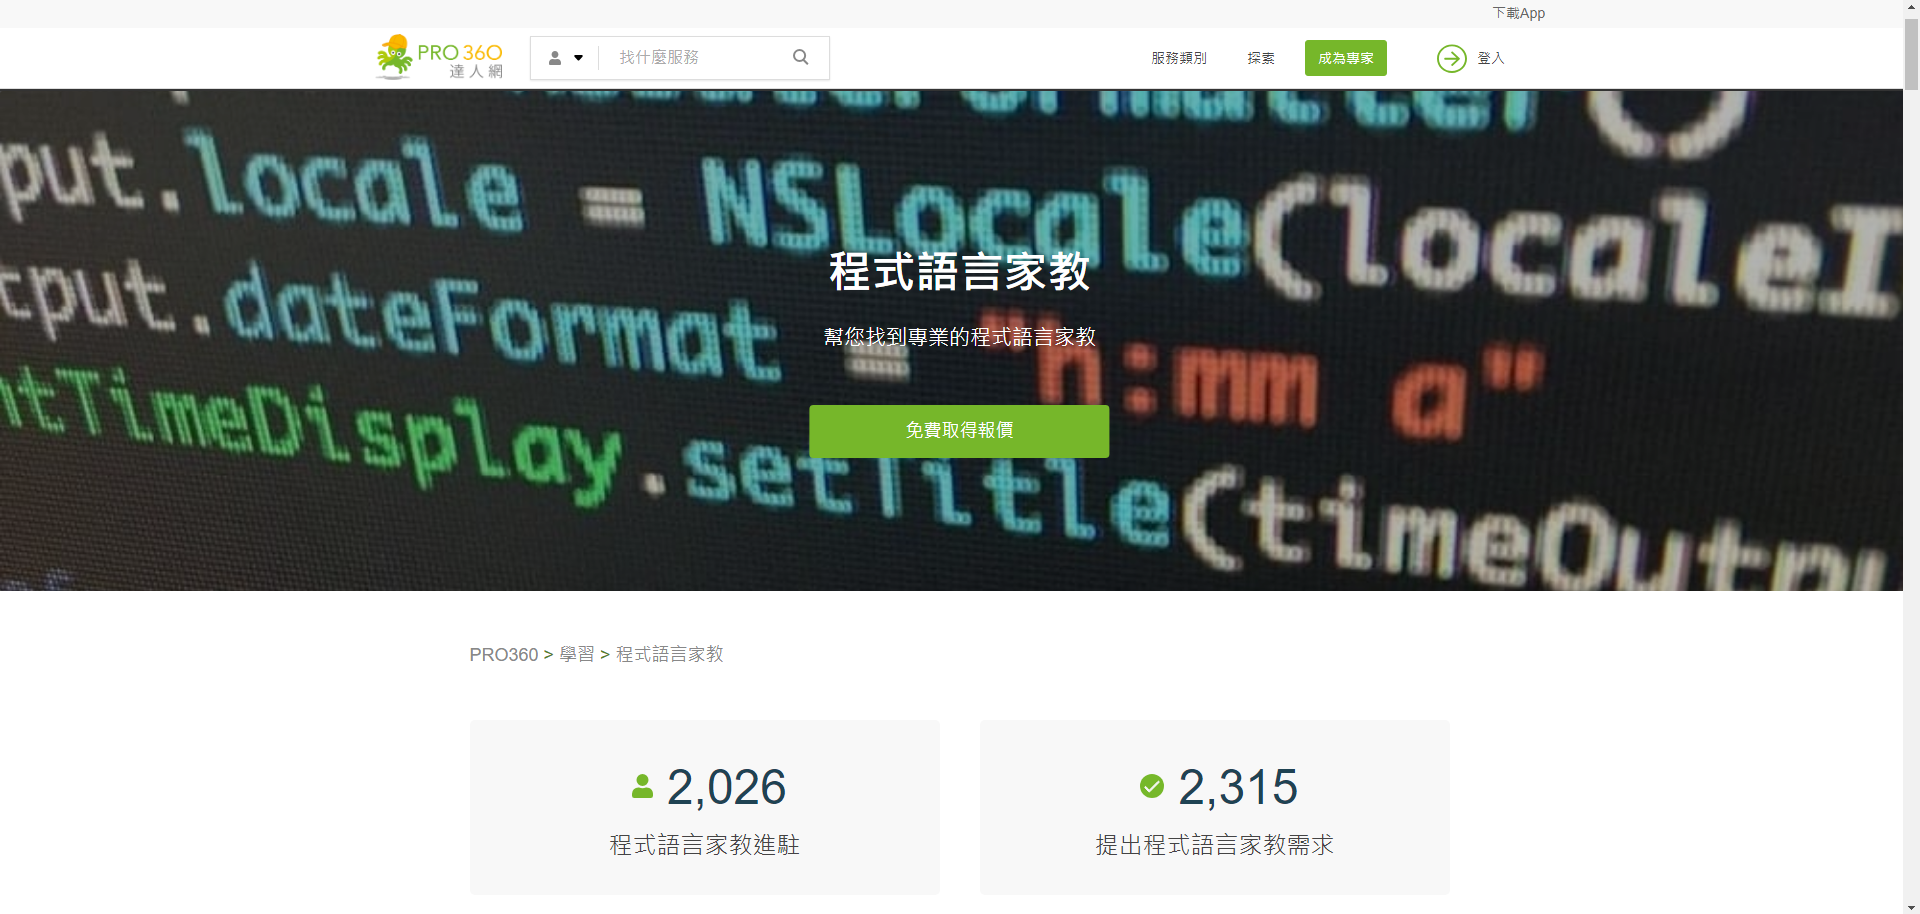
\includegraphics[width=1\textwidth]{images/pro360-2026.png}
		\caption{PRO360達人網}
		\label{fig:Teacher-3}
	\end{subfigure}
	\caption[各平台教師數量]{各平台教師數量\\(資料來源:於2024年2月22日,截取自AmazingTalker、1111家教網及PRO360達人網)}
\end{figure}

\subsection{線上教學平台分潤比例}
\label{fig:Appendix-profit-sharing}
% 兩張圖
\begin{figure}[H]
	\centering
	\begin{subfigure}{0.45\linewidth}
		\centering
		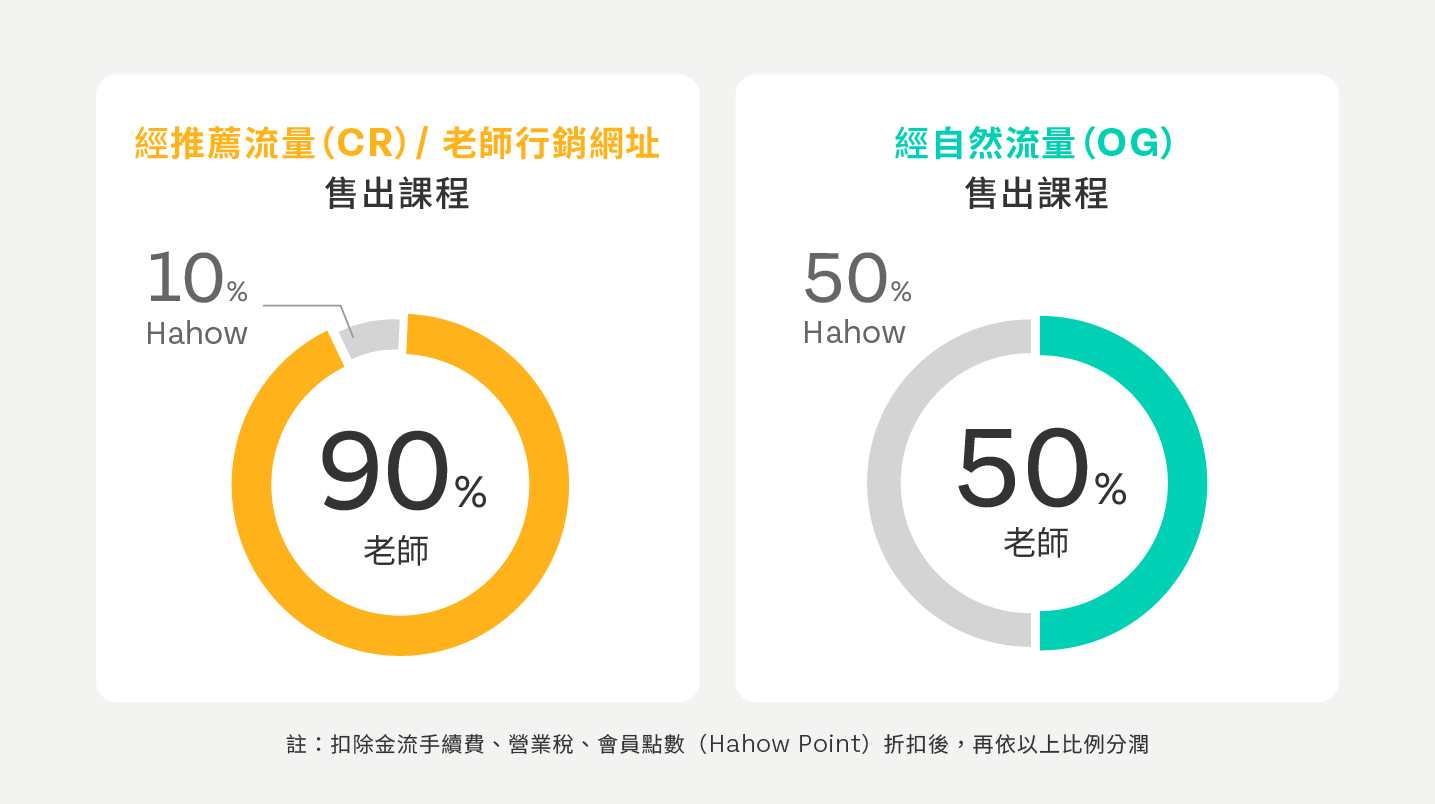
\includegraphics[width=1\textwidth]{images/hahow.png}
		\caption{Hahow好學校}
		\label{fig:Hahow}
	\end{subfigure}
	\begin{subfigure}{0.45\linewidth}
		\centering
		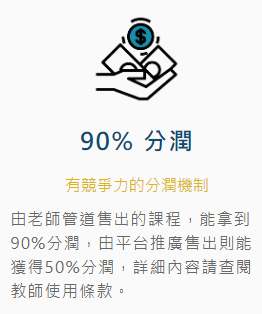
\includegraphics[width=0.6\textwidth]{images/hiskio.png}
		\caption{HiSKIO 專業線上教學平台}
		\label{fig:HiSKIO}
	\end{subfigure}
	\caption[線上教學平台分潤比例]{線上教學平台分潤比例\\(資料來源:於2024年2月22日,截取自Hahow好學校及HiSKIO 專業線上教學平台)}
\end{figure}

\newpage
\section{\centering 附件}
